\documentclass{nature3}
\usepackage{graphicx}
\usepackage{float}
\usepackage{verbatim}
\usepackage{hyperref}
\usepackage{amsmath}
\usepackage{amssymb}
\usepackage{aas_macros_nature}
\usepackage{lineno}

\linespread{1.0}
\linenumbers % turn line numbering on or off

\newcommand{\starname}{TIC 141146667}

\newcommand{\farcm}{\mbox{\ensuremath{.\mkern-4mu^\prime}}}%    % fractional arcminute symbol: 0.'0
\newcommand{\farcs}{\mbox{\ensuremath{.\!\!^{\prime\prime}}}}%  % fractional arcsecond symbol: 0.''0

\newcommand{\kms}{\ensuremath{\rm km\,s^{-1}}}
\newcommand{\ms}{\ensuremath{\rm m\,s^{-1}}}

\renewcommand*{\thefootnote}{\fnsymbol{footnote}}

%%%%%%%%%%%%%%%%
% INSTITUTIONS %
%%%%%%%%%%%%%%%%
\newcommand{\carnegie}{Observatories of the Carnegie Institution for Science, Pasadena, CA 91101, USA}
%%%%%%%%%%%%%%%%

%%%%%%%%%%
% VALUES %
%%%%%%%%%%
% NOTE: might need to be ingested before submission 
\newcommand{\stteff}{YYYY}
\newcommand{\stagemyr}{40}
\newcommand{\periodhr}{3.930}


%%%%%%%%%%%%%%%%%%%%%%%%%%%%%%%%%%%%%%%%%%
%%%%%%%%%%%%%%%%%%%%%%%%%%%%%%%%%%%%%%%%%%

\title{A Plasma Torus Around a Young Low-Mass Star}

\begin{document}

\author{Luke G. Bouma$^{1,2}$}

\maketitle

\scriptsize
\begin{affiliations}
\item \carnegie
\item Carnegie Fellow
\end{affiliations}
\normalsize

%%%%%%%%%%%%%%%%%%%%%%%%%%%%%%%%%%%%%%%%%%%%%%%%%%%%%%%%%%%%%%%%%%%%%%%%%%%%%%%
%%%%%%%%%%%%%%%%%%%%%%%%%%%%%%%%%%%%%%%%%%%%%%%%%%%%%%%%%%%%%%%%%%%%%%%%%%%%%%%

\begin{abstract}
\normalfont
Approximately one percent of red dwarfs younger than 100 million years
show structured, periodic optical light curves suggestive of transiting
clumps of opaque circumstellar material that corotate with the star
\cite{Rebull2016,Stauffer2017,Rebull2018,Bouma2024}.  The composition,
origin, and even the existence of this material are uncertain. The main
alternative hypothesis is that these stars are explained by complex
distributions of dark starspots or bright faculae distributed across
their surfaces \cite{Koen2021}.  Here, we present time-series
spectroscopy and photometry of a \stagemyr\ million year old complex
periodic variable (CPV), TIC 141146667. The spectra show coherent
sinusoidal Balmer emission at up to four times the star's equatorial
velocity, demonstrating the presence of extended clumps of circumstellar
plasma --- a plasma torus. These data rule out ``starspot-only'' and
``dust-only'' origin scenarios for CPVs, instead supporting either a
purely stellar origin for the phenomenon or extrinsic scenarios
involving long-lived disks or outgassing rocky bodies capable of
supplying sufficient gas.  Given that long-lived condensations of cool
($10^4$ K) plasma can persist in the hot ($10^6$ K) coronae of stars
with a wide range of masses
\cite{CollierCameron1989,Townsend2005,Dunstone2006,Petit2013,Waugh2022,Daley-Yates2024},
these data support the idea that such condensations can become optically
thick around the lowest-mass stars, although the exact source of 
opacity remains unclear.
\end{abstract}

\maketitle

%%%%%%%%%%%%%%%%%%%%%%%%%%%%%%%%%%%%%%%%%%%%%%%%%%%%%%%%%%%%%%%%%%%%%%%%%%%%%%%
%%%%%%%%%%%%%%%%%%%%%%%%%%%%%%%%%%%%%%%%%%%%%%%%%%%%%%%%%%%%%%%%%%%%%%%%%%%%%%%

\section{Main}
\label{sec:main}

\subsection{Introduction}

Lorem ipsum whatever...

\begin{figure}[t]
\centering
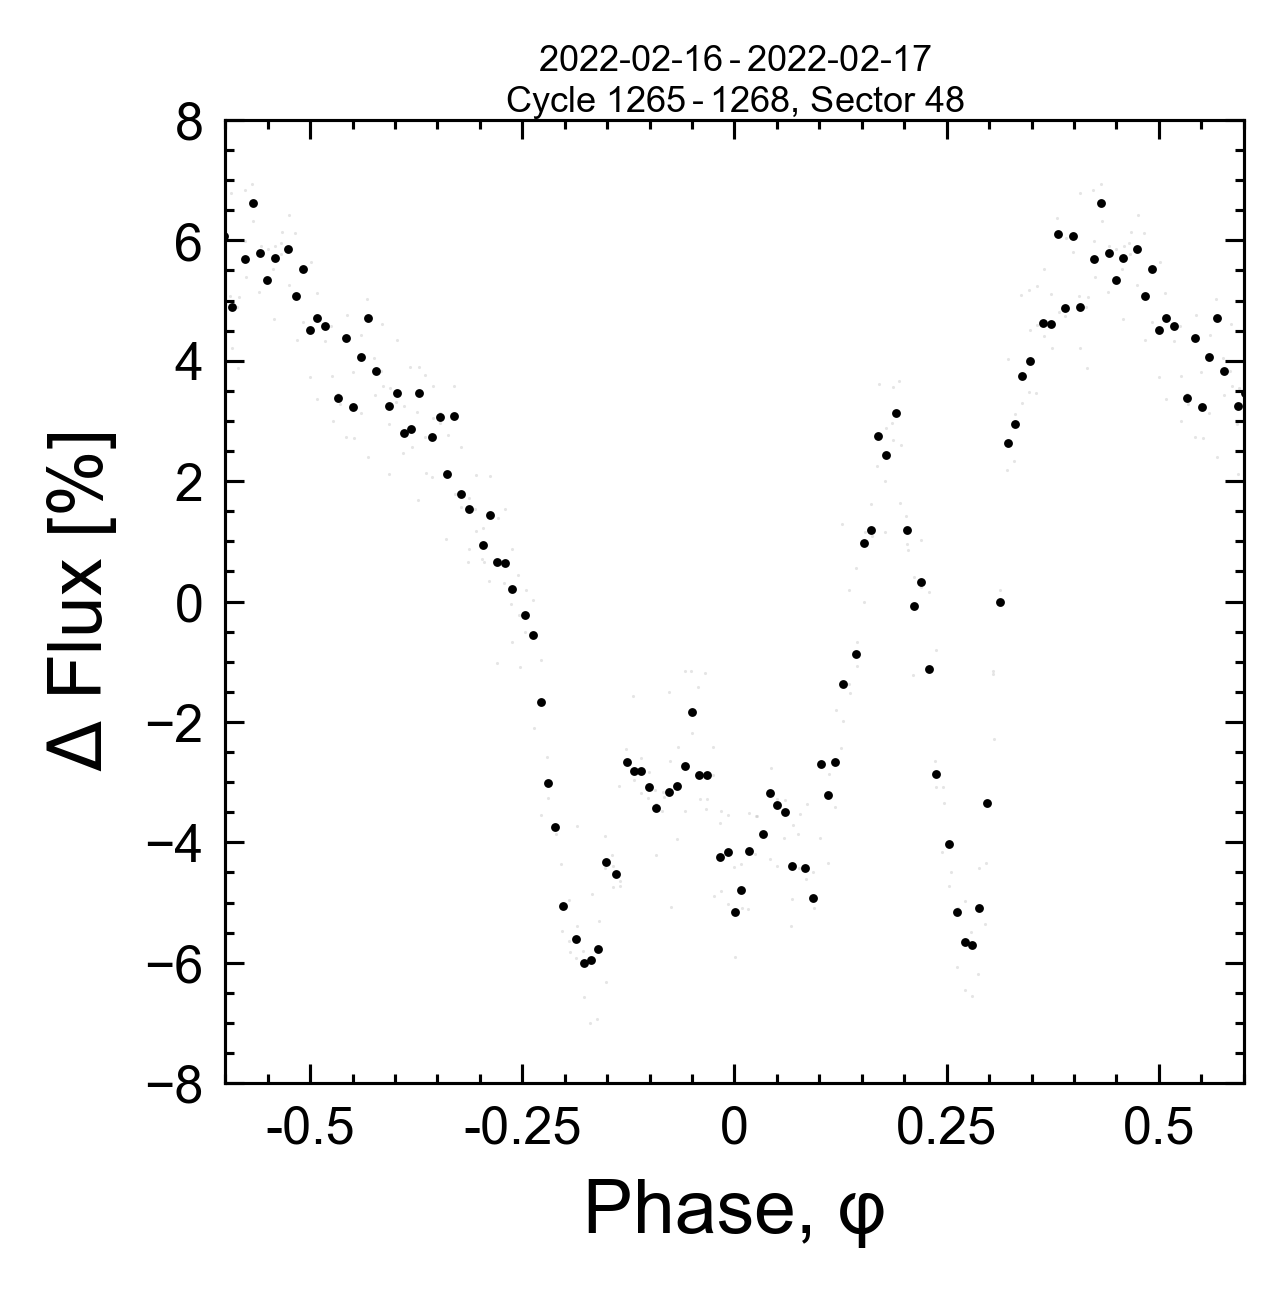
\includegraphics[width=0.7\textwidth]{figures/f1.png}
\caption[]{{\bf Figure 1 (Movie):  TIC 141146667 is a complex periodic
variable (CPV).} For the best experience, please view the online movie
available
\href{https://lgbouma.com/movies/movie_TIC1411_flux_phase.mp4}{here},
which spans a baseline of 5{,}784 cycles irregularly sampled over three
years.  The TESS light curve is phased to the \periodhr\ hour period in
groups of a few cycles per frame.  Raw data acquired with two minute
sampling are in gray; black is their average.  Similar to other members
of this class, the sharp photometric features persist for tens to
thousands of rotational cycles. }
\label{fig:lc}
\end{figure}


\subsection{Results}



\begin{figure}[t]
\centering
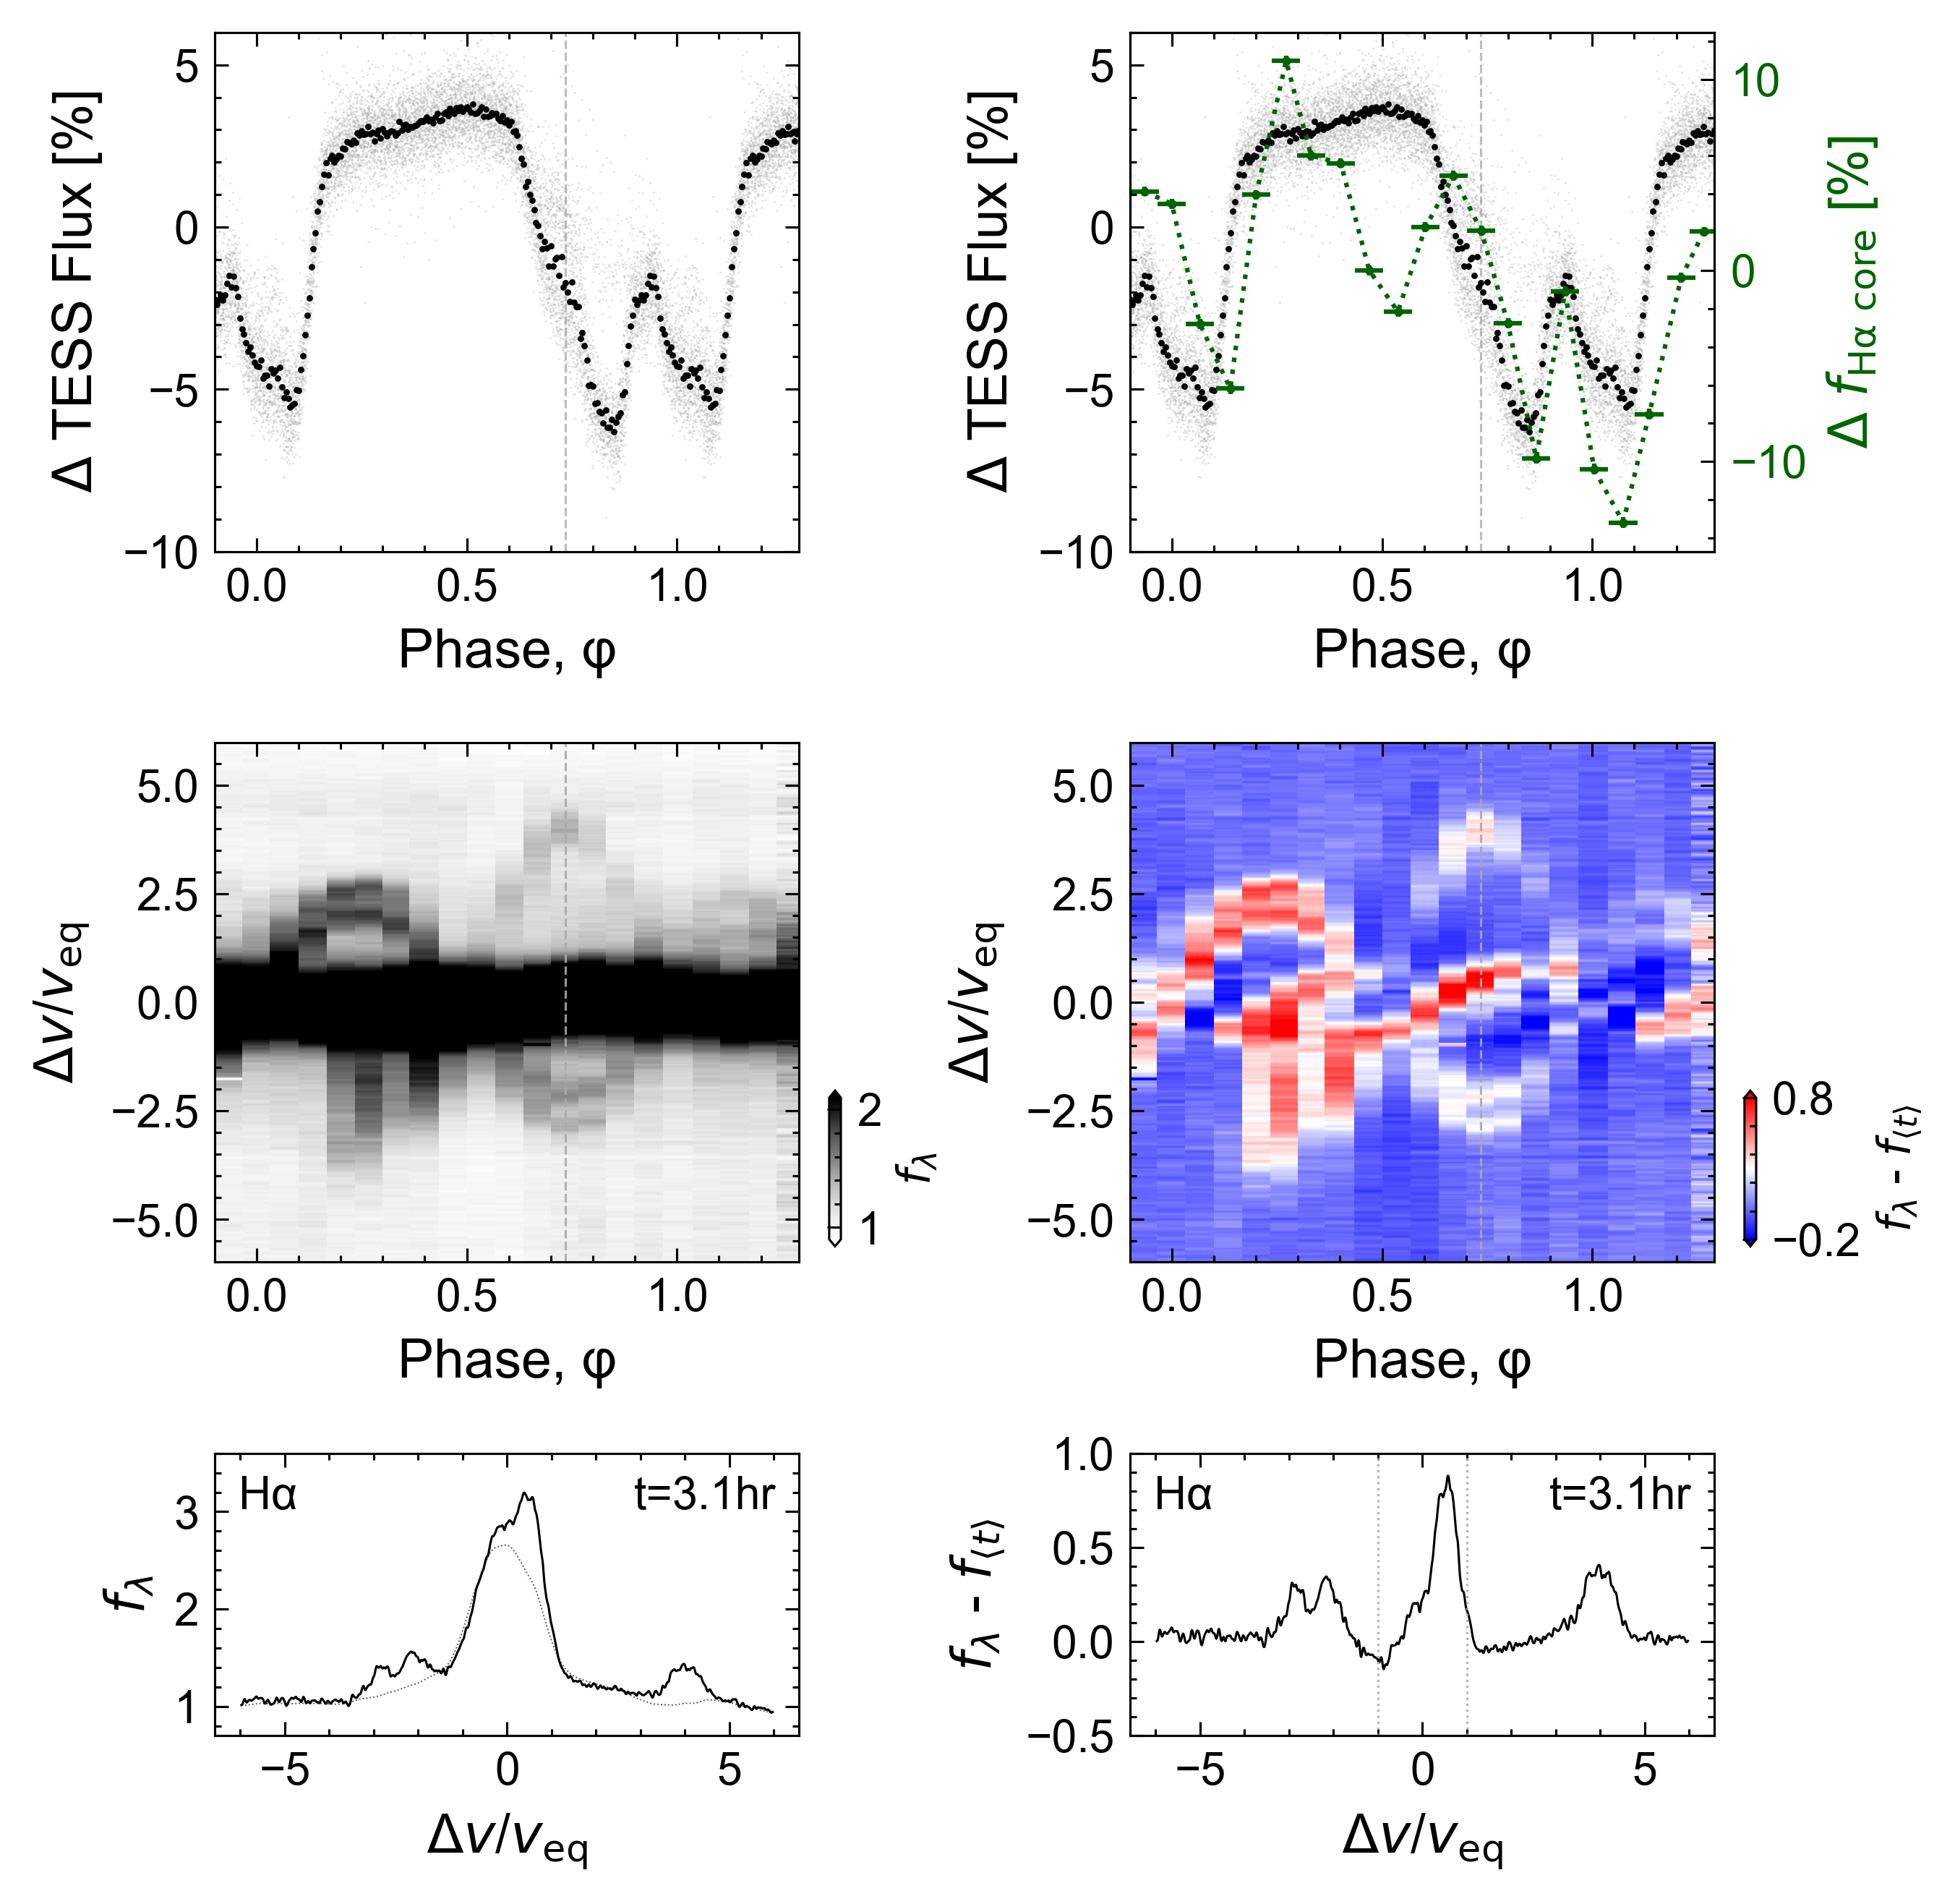
\includegraphics[width=0.99\textwidth]{figures/f2.png}
\caption[]{{\bf Figure 2 (Movie):}  
  Hydrogen emission from circumstellar plasma orbiting TIC 141146667.
  {(\bf TODO)}For the best experience, please view the online movie
  available
  \href{https://lgbouma.com/movies/TIC141146667_sixpanel.mp4}{here}.
  {\bf Panel a:} TESS light curve from UT 2024-02-05 to UT
  2024-02-26 folded on the \periodhr\ hour period.  Black points are
  averaged; gray are the raw data.
  {\bf Panel b:} Keck/HIRES H$\alpha$ spectra
  acquired on UT 2024-02-17.  The continuum is set at unity, and the
  darkest color is set at twice the continuum to accentuate emission
  outside the line core ($|v/v_{\rm eq}|>1$, for $v_{\rm eq}$=130\,\kms).
  While emission in the line core originates in the stellar
  chromosphere, the sinusoidal emission features are most readily
  described by a warped plasma torus.
  {\bf Panel c:} Individual epochs of Panel b, visible in the
  online movie.  The dotted line shows a time-averaged spectrum,
  $f_{\langle t \rangle}$.
  {\bf Panel d:} As in Panel a, but overplotting the
  median-normalized H$\alpha$ light curve at $|v/v_{\rm eq}|<1$.
  {\bf Panel e:} As in Panel b, after subtracting the time-averaged
  spectrum. In addition to circumstellar emission, the line core shows
  absorption during the plasma clump transits.  The asymmetric stretch
  is set to match the dynamic range of the data.
  {\bf Panel f:} Individual epochs of Panel e, visible in the online
  movie.}
\label{fig:spec}
\end{figure}


\subsection{Discussion}


%%%%%%%%%%%%%%%%%%%%%%%%%%%%%%%%%%%%%%%%%%%%%%%%%%%%%%%%%%%%%%%%%%%%%%%%%%%%%%%
%%%%%%%%%%%%%%%%%%%%%%%%%%%%%%%%%%%%%%%%%%%%%%%%%%%%%%%%%%%%%%%%%%%%%%%%%%%%%%%

\newpage
\begin{methods}

\renewcommand{\figurename}{Extended Data Figure}
\renewcommand{\tablename}{Extended Data Table}
\setcounter{table}{0}  
\setcounter{figure}{0}  


\subsection{Observations}

\subsection{Data Reduction}

\subsection{Modeling the Emitting Clump}


%%%%%%%%%%%%%%%%%%%%%%%%%
% Supplementary Figures %
%%%%%%%%%%%%%%%%%%%%%%%%%

%%%%%%%%%%%%%%%%%%%%%%%%
% Supplementary Tables %
%%%%%%%%%%%%%%%%%%%%%%%%

% TEMPLATE: IRAS041
%
\begin{table}
    \centering
    \begin{tabular}{lcr}
    \hline 
    \hline
    Parameter & Host & Source \\
    \hline 
    \multicolumn{3}{c}{Identifiers} \\
    \hline
    TIC & 141146667 & TESS \\
    Gaia & todo & Gaia\ DR3 \\
    %2MASS & J04154278+2909597 & J04154269+2909558 & 2MASS \\
    %ALLWISE & J041542.77+290959.5 & ... & ALLWISE\\
    \hline
    \multicolumn{3}{c}{Astrometry} \\ 
    \hline
    $\alpha$ & todo & Gaia\ DR3 \\
    $\delta$ & todo & Gaia\ DR3 \\
    $\mu_{\alpha}$ (mas yr$^{-1}$ ) & todo & Gaia\ DR3 \\
    $\mu_{\delta}$ (mas yr$^{-1}$ ) & todo & Gaia\ DR3 \\
    $\pi$ (mas) & todo & Gaia\ DR3 \\
    \hline
    \multicolumn{3}{c}{Photometry} \\
    \hline
    $TESS$ (mag) & todo & TESS\ \\
    $G$ (mag) & todo & Gaia\ DR3 \\
    $G_{\rm BP}$ (mag) & todo & Gaia\ DR3\\
    $G_{\rm RP}$ (mag) & todo & Gaia\ DR3\\
    $J$ (mag) & todo & 2MASS\\
    $H$ (mag) & todo & 2MASS\\
    $K_s$ (mag) & todo & 2MASS\\
    $W1$ (mag) & todo & ALLWISE \\
    $W2$ (mag) & todo & ALLWISE \\
    $W3$ (mag) & todo & ALLWISE \\
    $W4$ (mag) & todo & ALLWISE \\
    \hline
    \multicolumn{3}{c}{Kinematics and Position} \\
    \hline
    $RV_{Bary}$ (km s$^{-1}$ ) & $13.35 \pm 3.39$ & Gaia\ DR3 \\
    $U$ (km s$^{-1}$ ) & & \\
    $V$ (km s$^{-1}$ ) & & \\
    $W$ (km s$^{-1}$ ) & & \\
    $X$ (pc)  & & \\
    $Y$ (pc)  & & \\
    $Z$ (pc) & & \\
    \hline
    \multicolumn{3}{c}{Physical Properties} \\
    \hline
    $P_{rot}$ (hours) & $3.930 \pm 0.XXX$ & This work \\ 
    $v \sin i_\star$(km s$^{-1}$) & todo & This work\\
    $i_\star$($^\circ$) & todo & This work \\
    $F_{bol}$ (erg cm$^{-2}$ s$^{-1}$ ) & todo & This work\\
    $T_{eff}$ (K) & todo & This work\\
    $A_V$ (mag) & todo & This work \\
    $R_\star$ ($R_{\odot}$) & todo & This work\\
    $L_\star$ ($L_{\odot}$)  & todo & This work\\
    $M_\star$ ($M_{\odot}$)  & todo & This work\\
    Age (Myr) & todo &  This work \\
    \hline
    \end{tabular}
    \caption{Properties of \starname.}
    \label{tab:stellarParameters}
\end{table}


\end{methods}

\bibliography{cpvbib.bib} % common bib file
\bibliographystyle{naturemagfixed}   


\begin{addendum}

\item[Acknowledgments] The author thanks X, Y, Z.
  L.G.B. was suported by...
	Acknowledge TESS...


%TC:ignore
%% Author Contribution
\item[Author Contributions] ...
%TC:endignore

\item[Data Availability] ...

\item[Competing Interests] The authors declare that they have no competing
financial interests.
 
\item[Correspondence] Correspondence and requests for materials should be
addressed to ...
 
\item[Code availability] We provide access to a GitHub repository including all
code created for the analysis of this project that is not already publicly
available.

\end{addendum}



\end{document}


